
\subsection{Organisation.}
\begin{frame}
    \frametitle{Chaine de commande.}
    \only<1> {
        \input cmd.tex
    }
    \only<2> {
        \input cmd_log.tex
    }
\end{frame}

\begin{frame}
    \frametitle{La pandaboard.}
    \begin{center}
        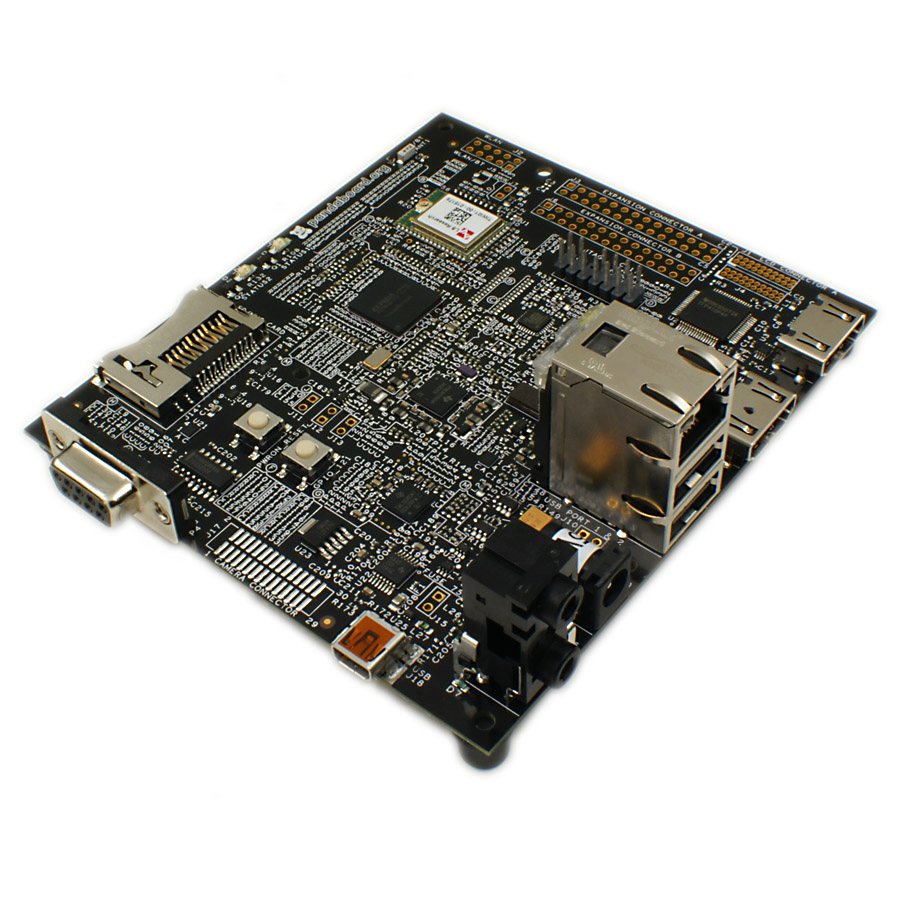
\includegraphics[scale=.15]{rcs/panda.png}
    \end{center}
    \uncover<2-> {
        Rôles : \begin{enumerate}
            \pause \item Détection d'obstacles.
            \pause \item Suivi de l'utilisateur.
            \pause \item Décision de la trajectoire.
        \end{enumerate}
    }
\end{frame}

\begin{frame}
    \frametitle{La caméra.}
    \begin{center}
        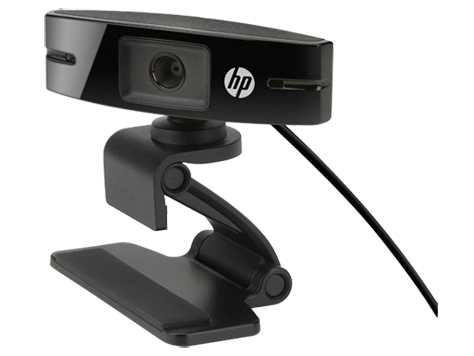
\includegraphics[width=0.8\linewidth]{rcs/cam.png}
    \end{center}
\end{frame}

\begin{frame}
    \frametitle{La carte arduino.}
    \begin{center}
        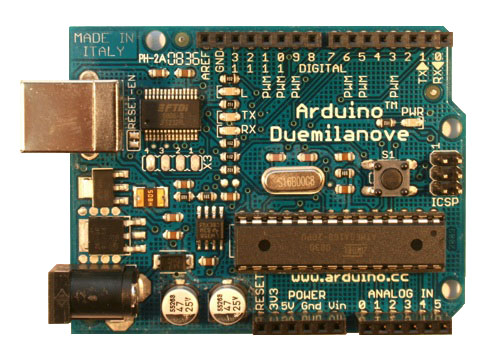
\includegraphics[scale=.3]{rcs/ardui.png}
    \end{center}
    \uncover<2-> {
        Rôles : \begin{enumerate}
            \pause \item Contrôle des moteurs.
            \pause \item Communication bluetooth.
            \pause \item Lien entre les différents composants.
        \end{enumerate}
    }
\end{frame}

\begin{frame}
    \frametitle{Le shield bluetooth.}
    \begin{center}
        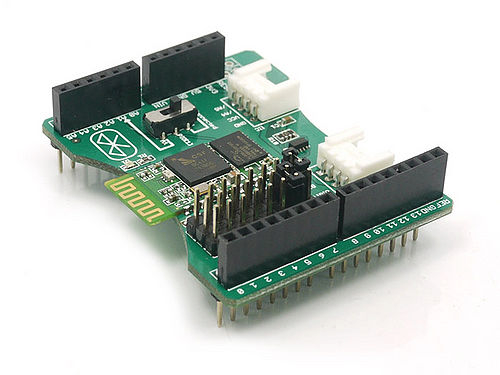
\includegraphics[width=0.8\linewidth]{rcs/btshield.png}
    \end{center}
\end{frame}

\subsection[Suivi]{Suivi de l'utilisateur.}
\begin{frame}
    \frametitle{Approche temporelle.}
    \framesubtitle{Situation initiale.}
    \only<1> {
        \begin{center}
            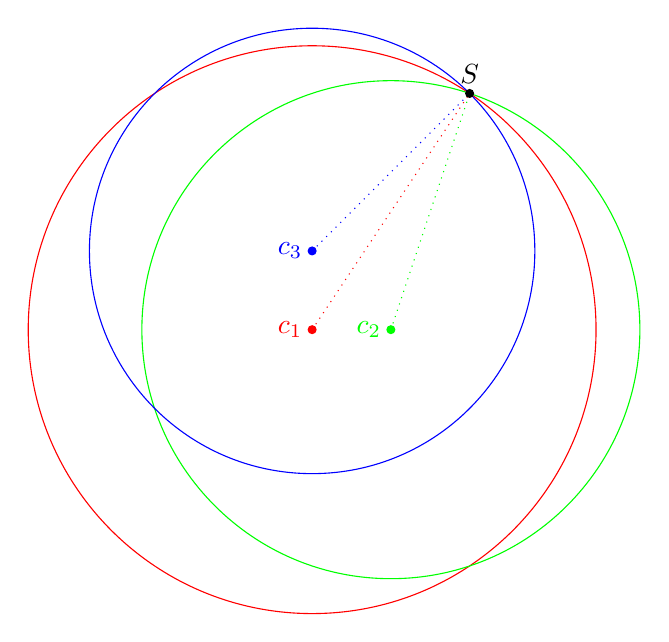
\begin{tikzpicture}
                \filldraw[red] (0,0) circle [radius=.05] node [left] {$c_1$};
                \filldraw[green] (1,0) circle [radius=.05] node [left] {$c_2$};
                \filldraw[blue] (0,1) circle [radius=.05] node [left] {$c_3$};
                \draw[red] (0,0) circle [radius=3.6056];
                \draw[green] (1,0) circle [radius=3.1623];
                \draw[blue] (0,1) circle [radius=2.8284];
                \draw[red,dotted] (0,0) -- (2,3);
                \draw[green,dotted] (1,0) -- (2,3);
                \draw[blue,dotted] (0,1) -- (2,3);
                \filldraw[black] (2,3) circle [radius=.05] node [above] {$S$};
            \end{tikzpicture}
        \end{center}
    }
    \only<2->{ \begin{block}{Équation de départ.}
            \begin{center}
                \begin{tabular}{rcl}
                    $(x-x_1)^2+(y-y_1)^2+(z-z_1)^2$ & $=$ & $d_1^2$ \\
                    $(x-x_2)^2+(y-y_2)^2+(z-z_2)^2$ & $=$ & $d_2^2$ \\
                    $(x-x_3)^2+(y-y_3)^2+(z-z_3)^2$ & $=$ & $d_3^2$ \\
                \end{tabular}
            \end{center}
    \end{block} }
    \only<3-> { \begin{block}{Positionnement des capteurs.}
            \begin{center}
                \begin{tabular}{rcl}
                    $(x_1;y_1;z_1)$ & $=$ & $(0;0;0)$ \\
                    $(x_2;y_2;z_2)$ & $=$ & $(d;0;0)$ \\
                    $(x_3;y_3;z_3)$ & $=$ & $(0;d;0)$ \\
                \end{tabular}
            \end{center}
    \end{block} }
\end{frame}

\begin{frame}
    \frametitle{Approche temporelle.}
    \framesubtitle{Résultats.}
    \begin{block}{Triangulation.}
        \begin{center}
            \begin{tabular}{rcl}
                $x$ & $=$ & $\frac{d_1^2-d_2^2+d^2}{2d}$ \\
                $y$ & $=$ & $-\frac{d_3^2-d_1^2-d^2}{2d}$ \\
                $z$ & $=$ & $\pm\sqrt{d_1^2-x^2-y^2}$ \\
            \end{tabular}
        \end{center}
    \end{block}
    \only<2-> {
        \begin{exampleblock}{Simulation.}
            \begin{itemize}
                \pause \item Ordre de grandeur des durées : $10^{-8}s$.
                \pause \item Précision temporelle nécessaire pour un positionnement à $50cm$ : $10^{-11}s$.
            \end{itemize}
        \end{exampleblock}
    }
\end{frame}

\begin{frame}
    \frametitle{Utilisation de l'intensité.}
    \begin{exampleblock}{Loi du carré inverse.}
        L'intensité d'un signal électromagnétique est inversement proportionnel au carré de la distance parcourue.
    \end{exampleblock}
    \only<2-> { \begin{block}{Lien entre distance et intensité.}
            \[ \frac{I_1}{I_2} = \frac{d_2^2}{d_1^2} \Leftrightarrow \frac{d_2}{d_1} = \sqrt{\frac{I_1}{I_2}} \]
    \end{block} }
\end{frame}

\begin{frame}
    \frametitle{Utilisation d'une caméra.}
    \begin{tabular}{cc}
        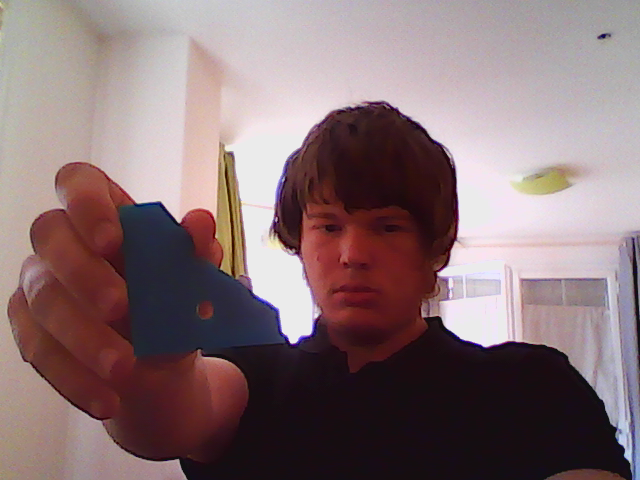
\includegraphics[width=.4\linewidth]{rcs/follow_bef.png} & 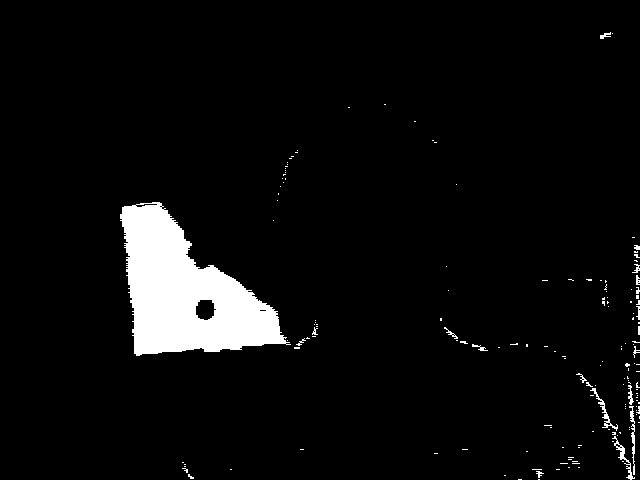
\includegraphics[width=.4\linewidth]{rcs/follow_aft.png} \\
    \end{tabular}
    \only<2-> { \begin{alertblock}{Limites}
            \begin{itemize}
                \pause \item L'utilisateur doit être dans le champ de vision du robot.
                \pause \item Il doit porter une couleur particulière.
                \pause \item Relativement sensible à l'éclairage.
                \pause \item Si la couleur est présente ailleurs sur le décor, le robot va être désorienté.
            \end{itemize}
    \end{alertblock} }
\end{frame}

\begin{frame}
    \frametitle{Espace de couleur \emph{HSV}.}
    \begin{center}
        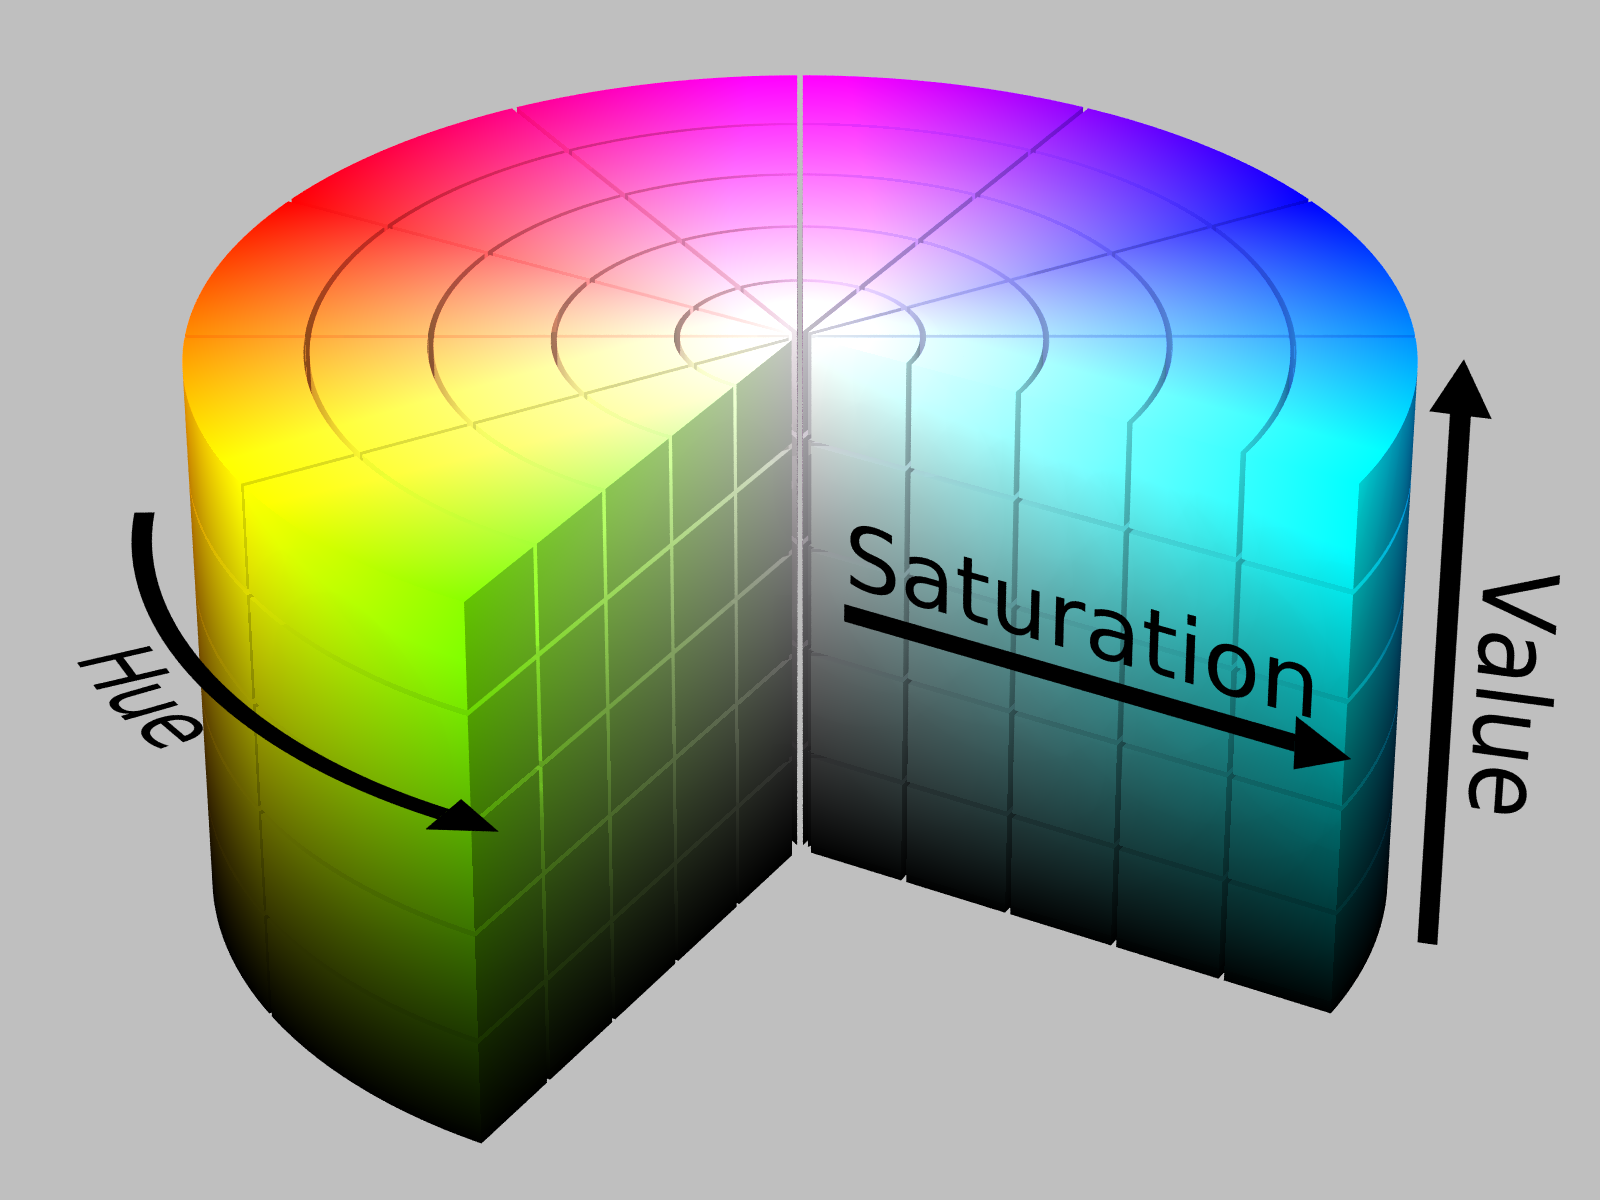
\includegraphics[width=.8\linewidth]{rcs/hsv.png}
    \end{center}
\end{frame}

\subsection[Obstacles]{Détection des obstacles.}
\begin{frame}
    \frametitle{Stéréovision.}
    \framesubtitle{Principe.}
    \begin{tabular}{cc}
        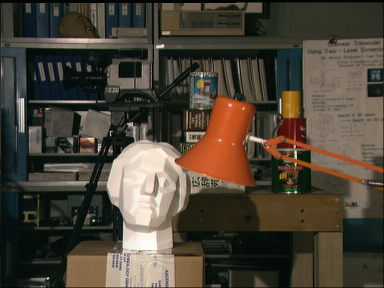
\includegraphics[width=.4\linewidth]{rcs/tsukuba.png} & 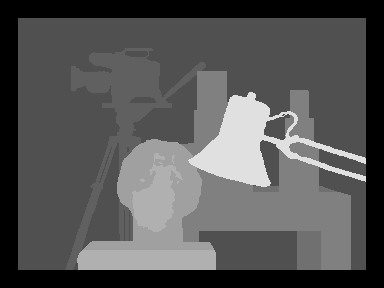
\includegraphics[width=.4\linewidth]{rcs/tsukuba_disp.png} \\
    \end{tabular}
    \only<2-3> { \begin{exampleblock}{Avantages}
            \begin{itemize}
                \pause \item Détecte tous les obstacles dans le champ de vision de la caméra.
                \pause \item Efficace contre les obstacles de type \emph{coin de table}.
            \end{itemize}
    \end{exampleblock} }
    \only<4-> { \begin{alertblock}{Limites}
            \begin{itemize}
                \pause \item Calculatoire et complexe.
                \pause \item Nécessite une unité de calcul puissante : coût élevé.
            \end{itemize}
    \end{alertblock} }
\end{frame}

\begin{frame}
    \frametitle{Stéréovision.}
    \framesubtitle{Résultats.}
    \begin{tabular}{ccc}
        \textbf{Caméra gauche} & \textbf{Caméra droite} & \textbf{Carte de disparité} \\
        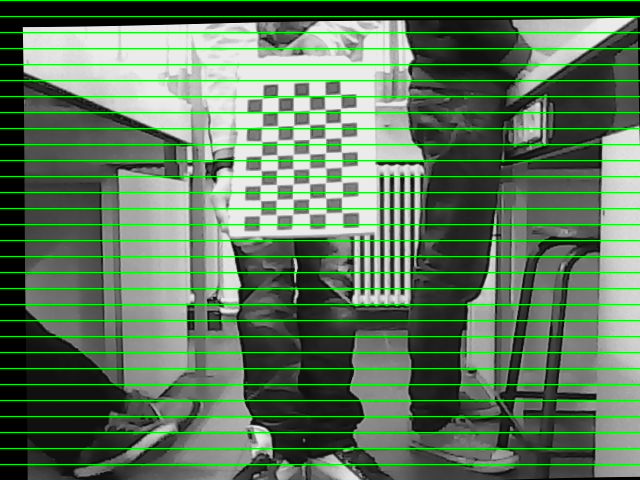
\includegraphics[width=0.3\linewidth]{rcs/rem0l.png} & 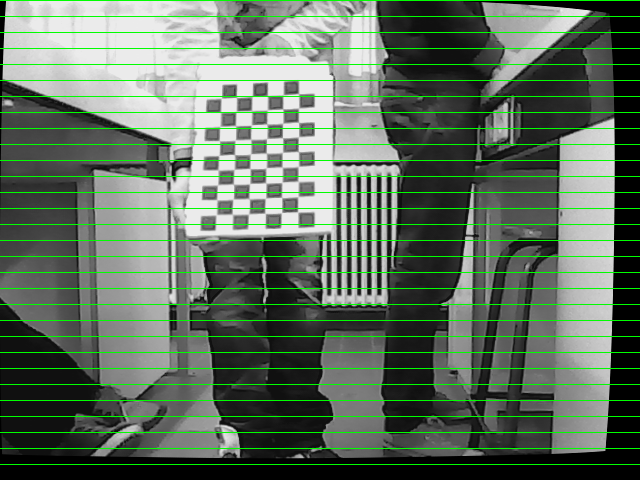
\includegraphics[width=0.3\linewidth]{rcs/rem0r.png} & 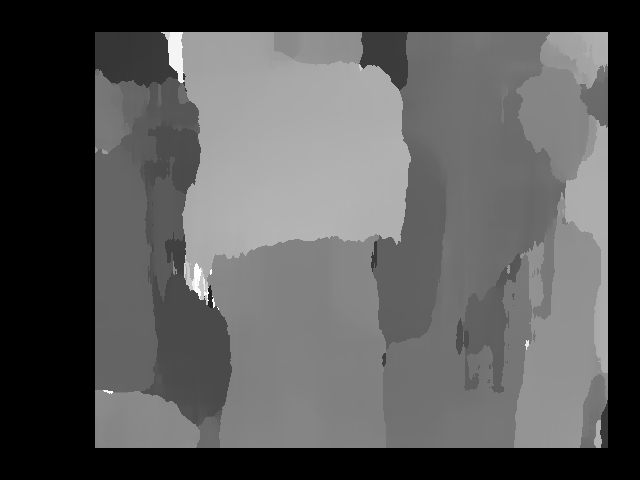
\includegraphics[width=0.3\linewidth]{rcs/disp0.png} \\
        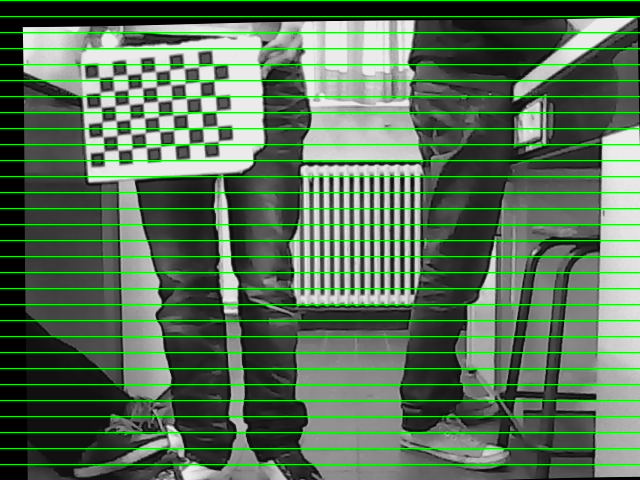
\includegraphics[width=0.3\linewidth]{rcs/rem1l.png} & 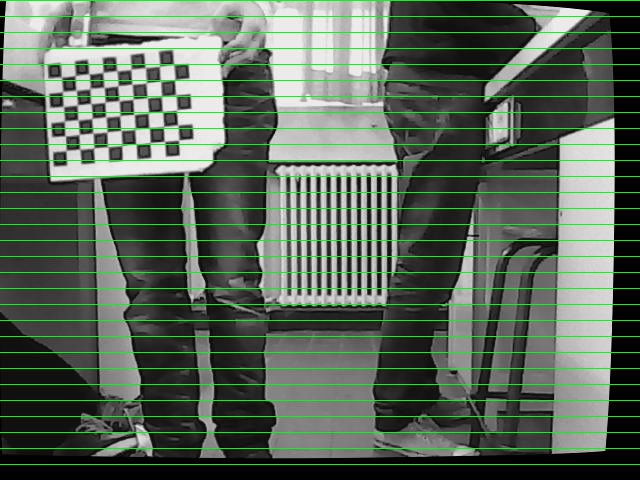
\includegraphics[width=0.3\linewidth]{rcs/rem1r.png} & 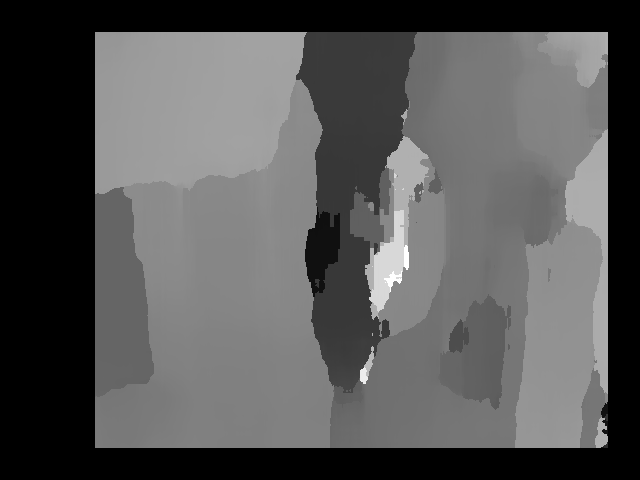
\includegraphics[width=0.3\linewidth]{rcs/disp1.png} \\
        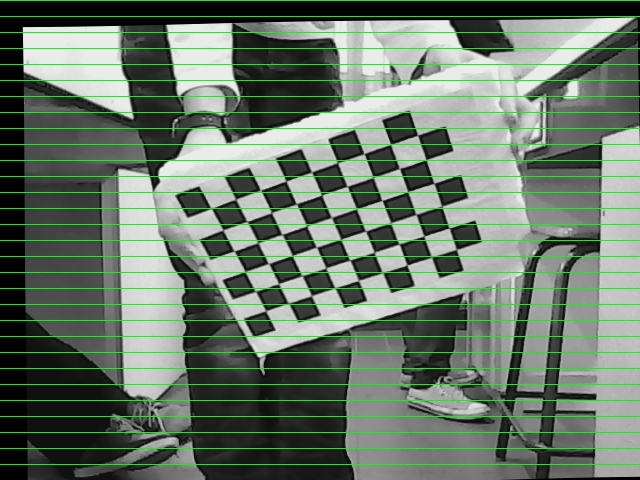
\includegraphics[width=0.3\linewidth]{rcs/rem2l.png} & 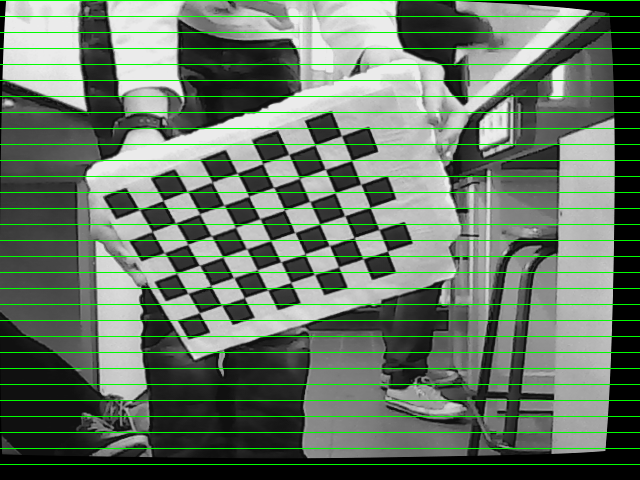
\includegraphics[width=0.3\linewidth]{rcs/rem2r.png} & 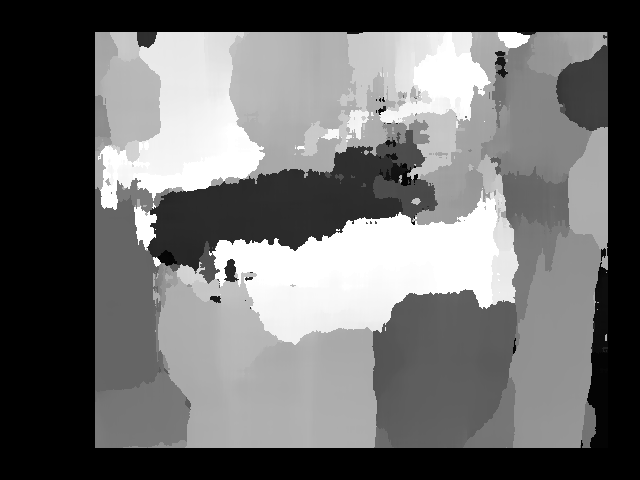
\includegraphics[width=0.3\linewidth]{rcs/disp2.png} \\
    \end{tabular}
\end{frame}

\begin{frame}
    \frametitle{Approche \emph{ABOD}.}
    \framesubtitle{Principe.}
    \only<1> {
        \begin{center}
            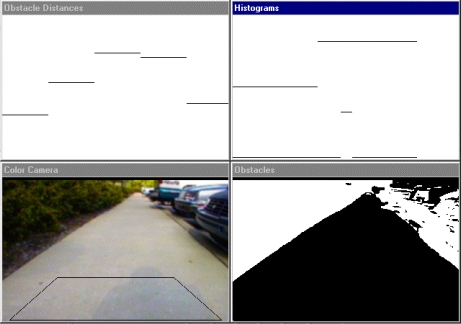
\includegraphics[width=0.8\linewidth]{rcs/abod.png}
        \end{center}
    }
    \only<2-> {
        \begin{alertblock}{Limites}
            \begin{itemize}
                \pause \item Le sol doit être globalement uni et différent des obstacles.
                \pause \item Inefficace contre les obstacles de type \emph{coin de table}.
                \pause \item Sans être aussi calculatoire que la stéréovision, nécessite une unité de calcul puissante.
                \pause \item A une période d'apprentissage : ne peut pas fonctionner dans un environnement inconnu.
            \end{itemize}
        \end{alertblock}
    }
\end{frame}

\begin{frame}
    \frametitle{Approche \emph{ABOD}.}
    \framesubtitle{Simulation.}
    \begin{center}
        \only<1> {
            \begin{tabular}{cc}
                \textbf{Caméra} & \textbf{Résultat} \\
                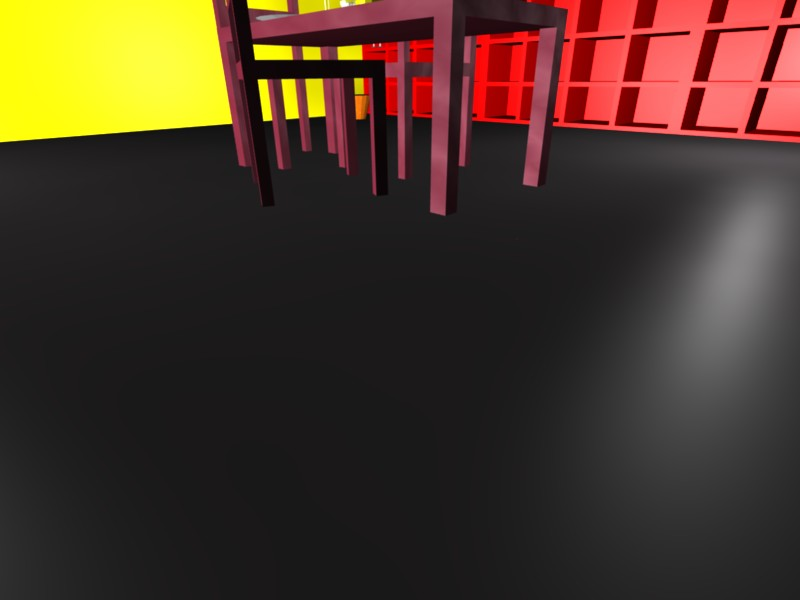
\includegraphics[width=0.4\linewidth]{rcs/abodv0s.png} & 
\includegraphics[width=0.4\linewidth]{rcs/abodv0r.png} \\
            \end{tabular}
            \begin{block}{Détails}
                \begin{itemize}
                    \item Indique $75\%$ de sol alors qu'il y en a $76.5\%$ : $1.7\%$  du sol est annoncé comme obstacle.
                    \item Indique $25\%$ d'obstacles alors qu'il y en a $23.5\%$ : $0.1\%$ des obstacles sont anoncés comme faisant partie du sol.
                \end{itemize}
            \end{block}
        } \only<2> {
            \begin{tabular}{cc}
                \textbf{Caméra} & \textbf{Résultat} \\
                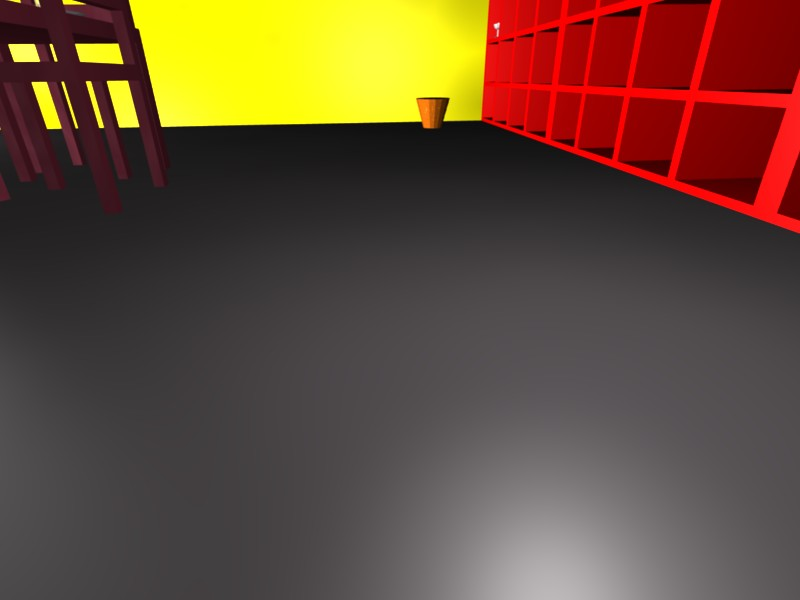
\includegraphics[width=0.4\linewidth]{rcs/abodv1s.png} & 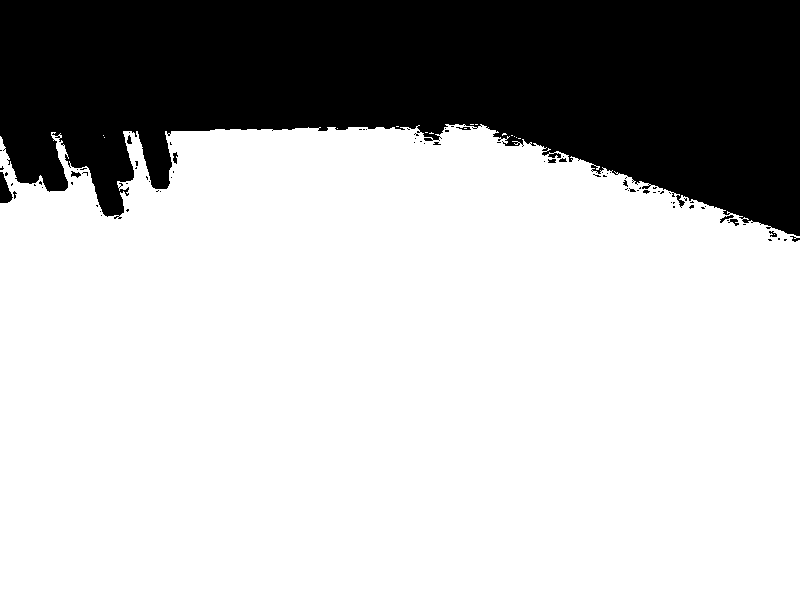
\includegraphics[width=0.4\linewidth]{rcs/abodv1r.png} \\
            \end{tabular}
            \begin{block}{Détails}
                \begin{itemize}
                    \item Indique $73\%$ de sol alors qu'il y en a $74.4\%$ : $1.7\%$  du sol est annoncé comme obstacle.
                    \item Indique $27\%$ d'obstacles alors qu'il y en a $25.6\%$ : tous les obstacles sont anoncés comme tel.
                \end{itemize}
            \end{block}
        } \only<3> {
            \begin{tabular}{cc}
                \textbf{Caméra} & \textbf{Résultat} \\
                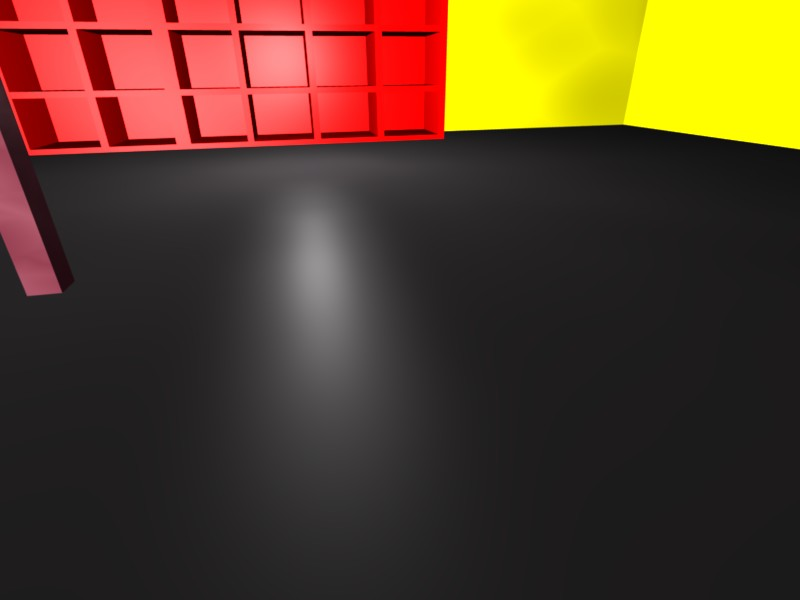
\includegraphics[width=0.4\linewidth]{rcs/abodv2s.png} & 
\includegraphics[width=0.4\linewidth]{rcs/abodv2r.png} \\
            \end{tabular}
            \begin{block}{Détails}
                \begin{itemize}
                    \item Indique $74.1\%$ de sol alors qu'il y en a $75.1\%$ : tout le sol est annoncé comme tel.
                    \item Indique $25.9\%$ d'obstacles alors qu'il y en a $24.9\%$ : $1.2\%$ des obstacles sont anoncés comme faisant partie du sol.
                \end{itemize}
            \end{block}
        }
    \end{center}
\end{frame}

\begin{frame}
    \frametitle{Approche \emph{ABOD}.}
    \framesubtitle{Résultats.}
    \begin{center}
        \only<1> {
            \begin{tabular}{cc}
                \textbf{Caméra} & \textbf{Résultat} \\
                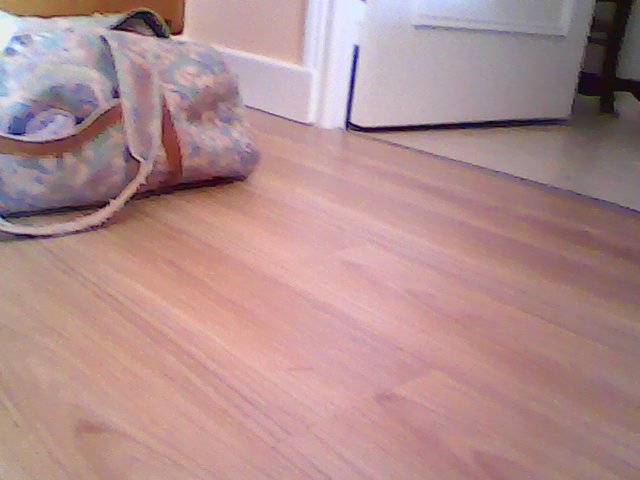
\includegraphics[width=0.4\linewidth]{rcs/abodr0s.png} & 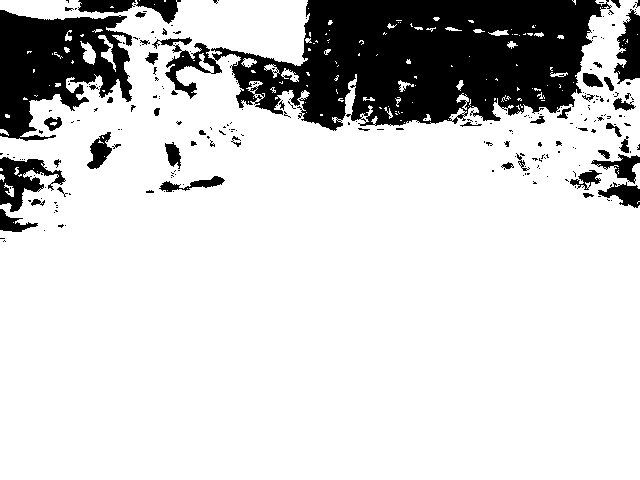
\includegraphics[width=0.4\linewidth]{rcs/abodr0r.png} \\
            \end{tabular}
            \begin{block}{Détails}
                \begin{itemize}
                    \item Indique $82\%$ de sol alors qu'il y en a $62.6\%$ : tout le sol est annoncé comme tel.
                    \item Indique $18\%$ d'obstacles alors qu'il y en a $37.4\%$ : $51.8\%$ des obstacles sont anoncés comme faisant partie du sol.
                \end{itemize}
            \end{block}
        } \only<2> {
            \begin{tabular}{cc}
                \textbf{Caméra} & \textbf{Résultat} \\
                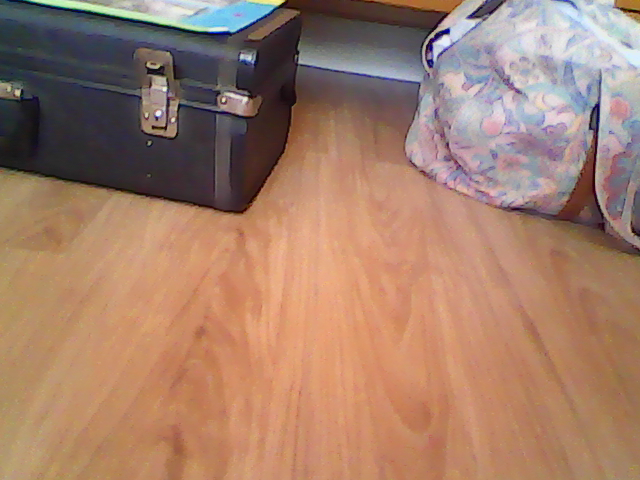
\includegraphics[width=0.4\linewidth]{rcs/abodr1s.png} & 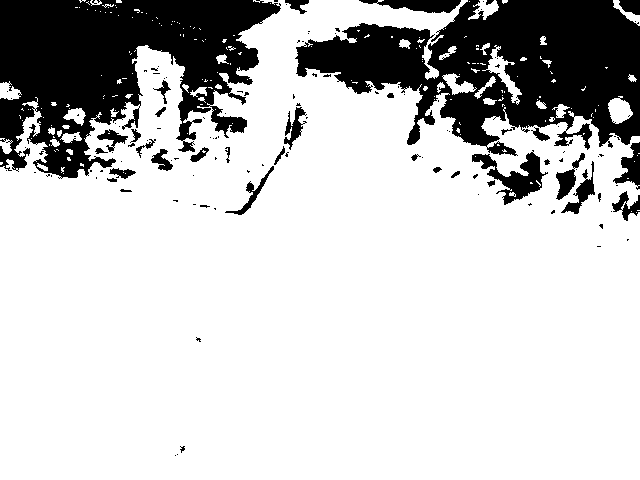
\includegraphics[width=0.4\linewidth]{rcs/abodr1r.png} \\
            \end{tabular}
            \begin{block}{Détails}
                \begin{itemize}
                    \item Indique $78.3\%$ de sol alors qu'il y en a $63.4\%$ : $0.7\%$  du sol est annoncé comme obstacle.
                    \item Indique $21.7\%$ d'obstacles alors qu'il y en a $36.6\%$ : $41.9\%$ des obstacles sont anoncés comme faisant partie du sol.
                \end{itemize}
            \end{block}
        }
    \end{center}
\end{frame}

